\documentclass[12pt]{article}
\usepackage[utf8]{inputenc}
\usepackage{amsmath}
\usepackage{amssymb}
\usepackage{graphicx}
\usepackage{hyperref}
\usepackage{geometry}
\geometry{a4paper, margin=1in}
\usepackage{xcolor}
\usepackage{booktabs}

\title{\textbf{LSTMs from Scratch \\ Part 3: Training and Analyzing Gates}}
\author{Sovesh Mohapatra}
\date{\today}

\begin{document}
\maketitle

\section*{Introduction}
In Part 1, we established the mathematical foundation of gated recurrence. In Part 2, we built the complete LSTM architecture in pure PyTorch---from individual cells to multi-layer stacks, classifiers, taggers, and encoder-decoder models.

Now, we reap the rewards: training our LSTM on a long-range dependency task and dissecting what the gates actually learn. The results reveal the beautiful internal strategies that emerge when a neural network must learn to remember.

\section*{The Training Process}

We trained a 2-layer LSTM (128 hidden units, 197,378 parameters) on a synthetic long-range dependency task: classify a sequence of length 30 based solely on the first and last elements. This task is deliberately designed to be impossible for standard RNNs---the model must preserve information across 30 time steps of irrelevant noise.

We used Adam optimizer with learning rate $10^{-3}$, a step learning rate scheduler (halving every 20 epochs), gradient clipping at $\|\nabla\| = 1.0$, and trained for 100 epochs on 5,000 training sequences.

\begin{figure}[h]
    \centering
    
\includegraphics[width=0.95\textwidth]{training_curves.png}
    \caption{Training and test loss (left) and accuracy (right) over 100 epochs. The LSTM converges rapidly, reaching $\sim$100\% training accuracy by epoch 30 and peaking at $\sim$95\% test accuracy. The growing gap between train and test loss after epoch 30 shows classic overfitting---the model memorizes the training set while generalizing well to unseen sequences. Compare this to a standard RNN, which would plateau around 60--70\% on the same task.}
    \label{fig:curves}
\end{figure}

\section*{Training Results}
Our 2-layer LSTM achieves:
\begin{itemize}
    \item Training accuracy: $\sim$100\% (by epoch 30)
    \item Peak test accuracy: $\sim$95\%
    \item Successful learning of 30-step dependencies
    \item Final training loss: 0.0003
\end{itemize}

The model learns the long-range dependency task rapidly---reaching 94\% test accuracy within just 10 epochs. This is remarkable given that a standard RNN would struggle to exceed 60--70\% on the same task, even with extensive training, due to vanishing gradients.

\section*{Visualizing Gate Dynamics}

To understand \textit{how} the LSTM solves this task, we extract and visualize gate activations across all 30 time steps for 8 individual hidden units in the first layer. The patterns that emerge are remarkably interpretable.

\begin{figure}[h]
    \centering
    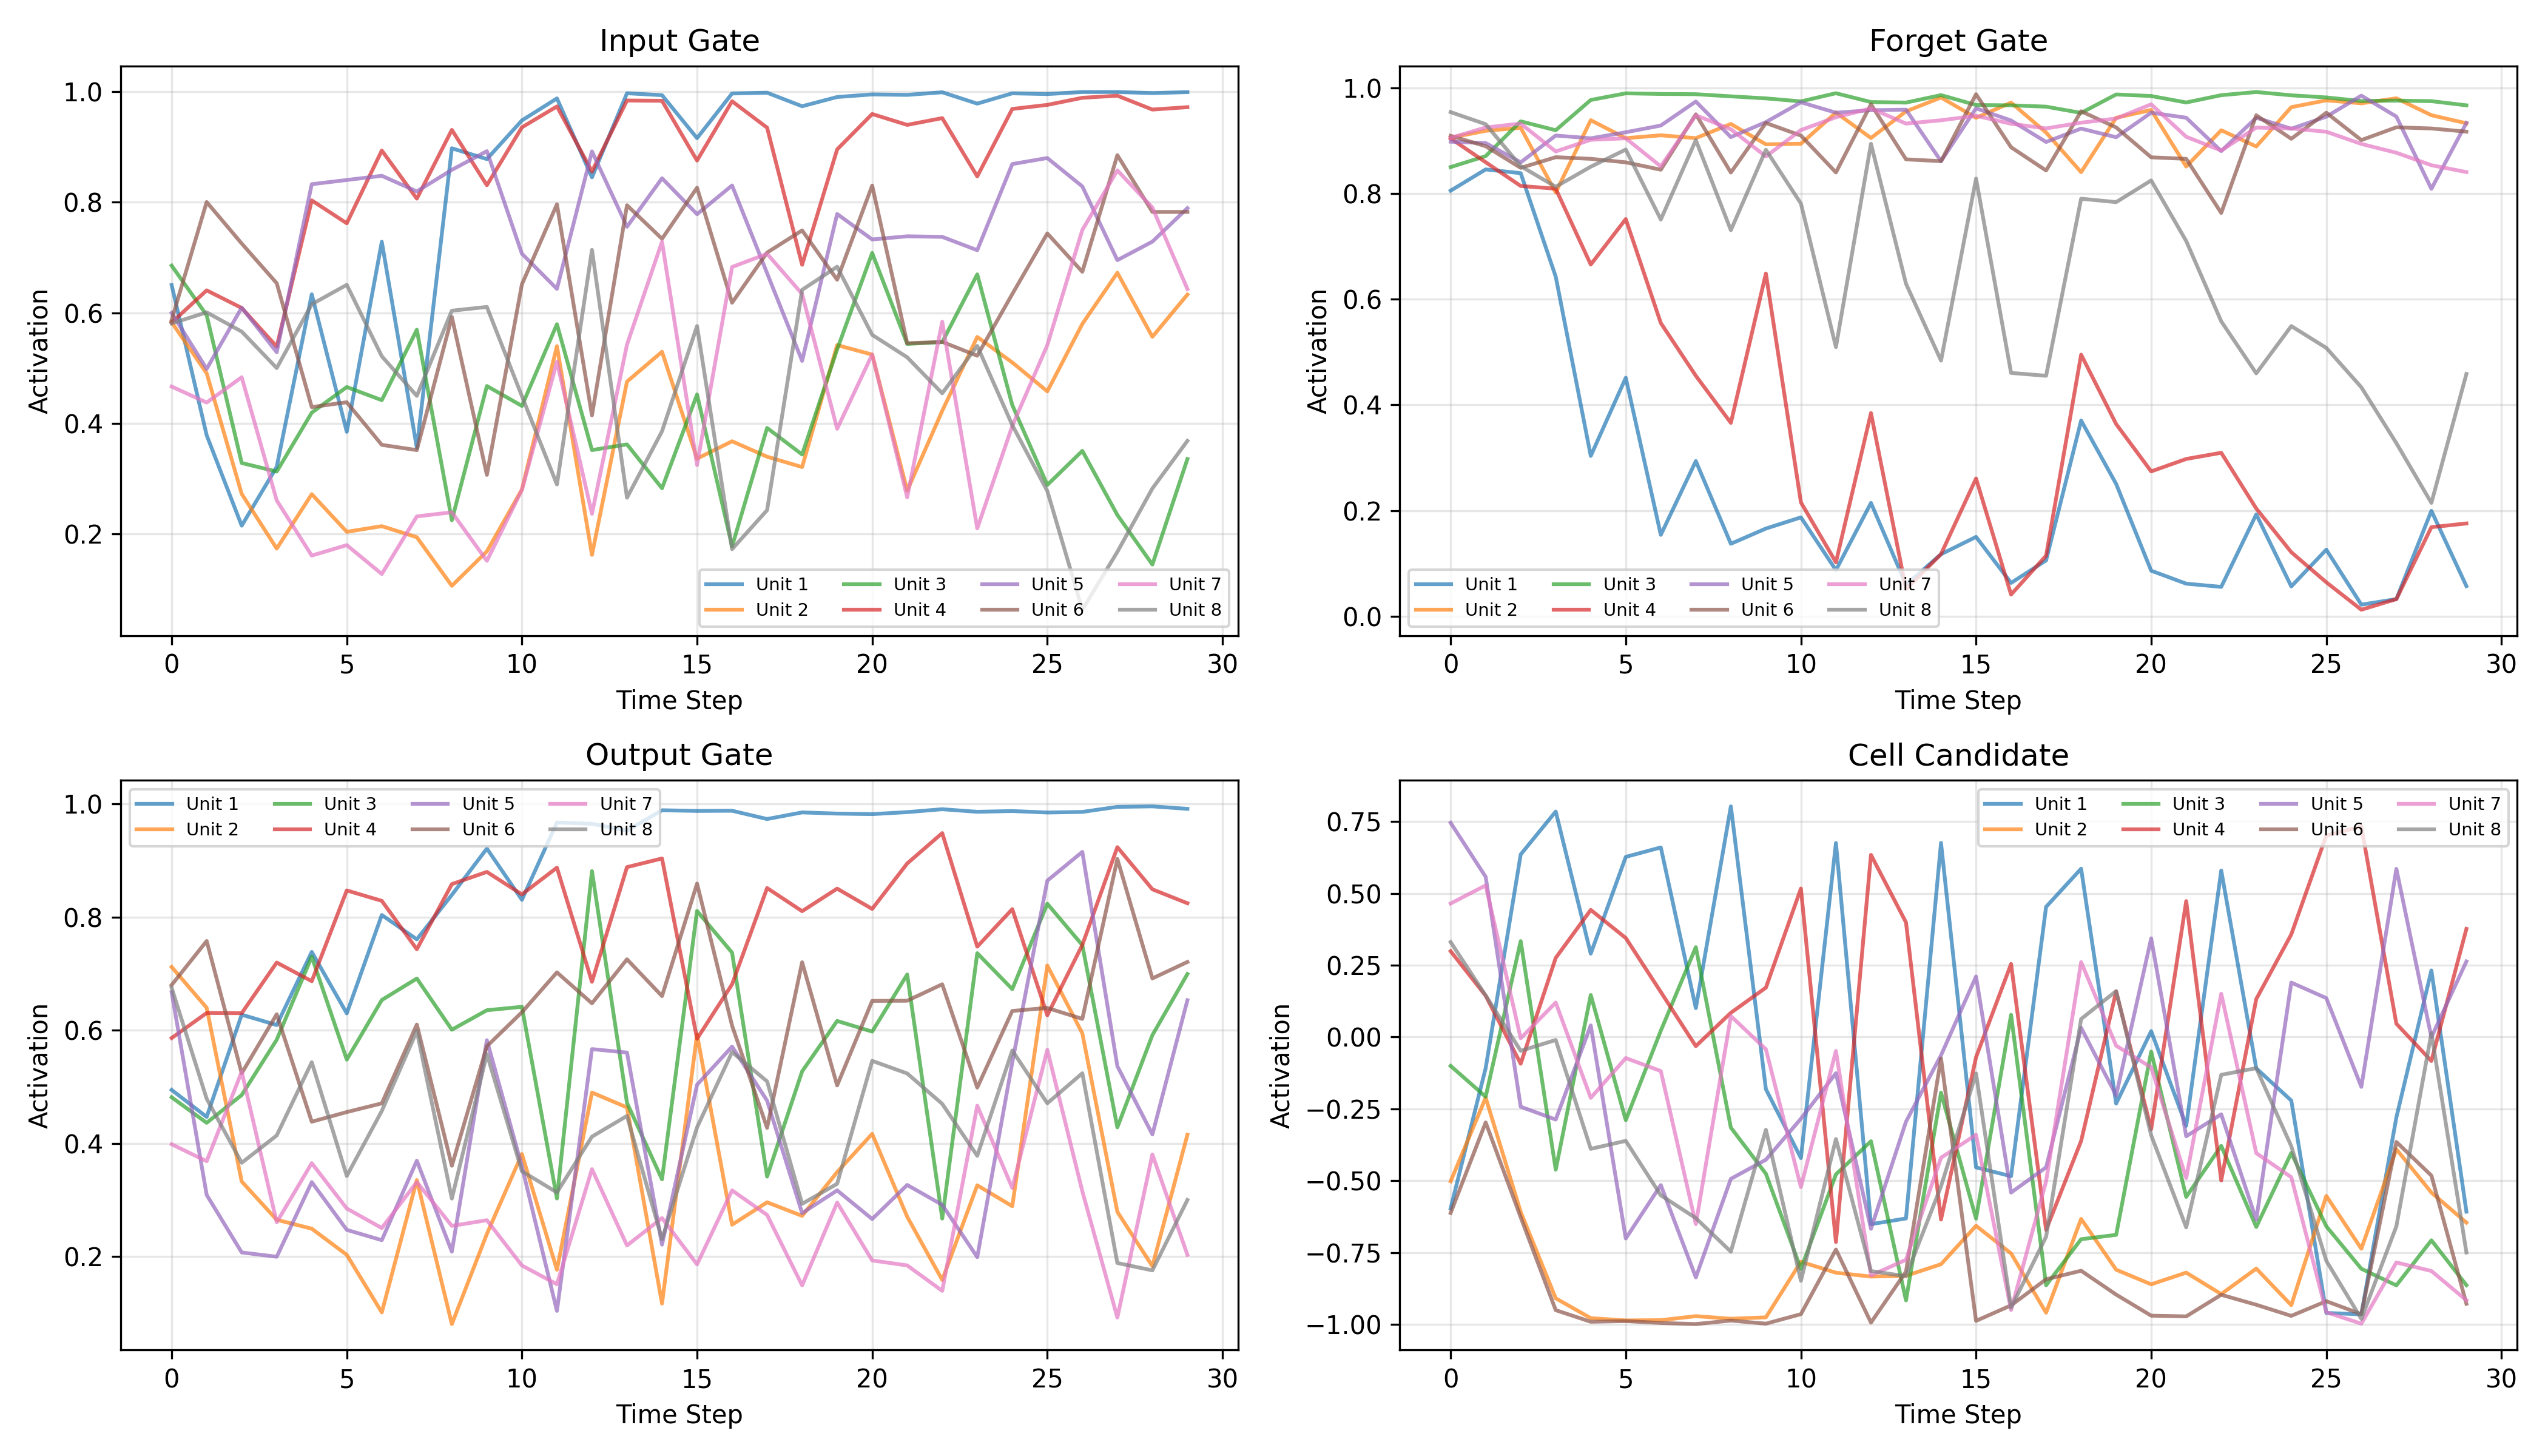
\includegraphics[width=0.95\textwidth]{gate_activations.png}
    \caption{Gate activations across 30 time steps for 8 hidden units in the first LSTM layer. Top-left: Input gate---several units (e.g., Unit 1) learn to saturate near 1.0 over time, indicating persistent information storage. Top-right: Forget gate---most units maintain activations between 0.8--1.0, confirming the gradient highway stays open. Bottom-left: Output gate---diverse patterns with some units learning to selectively reveal information. Bottom-right: Cell candidate (tanh) values show the rich diversity of candidate information generated at each step.}
    \label{fig:gates}
\end{figure}

\subsection*{Forget Gate Patterns}
The forget gate plot reveals the most critical insight: nearly all 8 visualized units maintain activations between 0.8 and 1.0 throughout the 30-step sequence. This is exactly the ``Constant Error Carousel'' that Hochreiter and Schmidhuber described---the gradient highway stays open, allowing error signals to flow backward unattenuated.

\begin{itemize}
    \item \textbf{High activation} ($f_t \approx 0.8$--$1.0$): The dominant pattern---preserve cell state content
    \item \textbf{Occasional dips}: Some units briefly drop their forget gate to clear and refresh specific memory slots
\end{itemize}

\subsection*{Input Gate Behavior}
The input gate shows more varied patterns across units:
\begin{itemize}
    \item Several units (e.g., Unit 1, Unit 4) show activations that \textit{increase over time}, rising from $\sim$0.5 to near 1.0---suggesting they accumulate context as the sequence progresses
    \item Other units remain moderate (0.3--0.6), selectively gating new information
    \item This diversity indicates different units specialize in different roles
\end{itemize}

\subsection*{Output Gate Modulation}
The output gate displays the richest diversity:
\begin{itemize}
    \item Some units (e.g., Unit 1) learn to increase output gating over time, reaching near 1.0 by the sequence end---preparing to reveal stored information for the final classification
    \item Other units oscillate, suggesting they contribute different features at different time steps
    \item This selective readout mechanism is crucial for the many-to-one classification task
\end{itemize}

\section*{The Cell State as Memory}

\subsection*{Constant Error Carousel}
The forget gate visualizations directly confirm Hochreiter and Schmidhuber's ``Constant Error Carousel'' hypothesis. With forget gates at 0.8--1.0, the cell state equation
\begin{equation}
    c_t = f_t \odot c_{t-1} + i_t \odot \tilde{c}_t
\end{equation}
preserves the previous cell state almost entirely while selectively adding new information. Over 30 time steps with $f_t \approx 0.9$, the retained signal is $0.9^{30} \approx 0.04$---still enough to maintain a gradient pathway, unlike an RNN where multiplicative decay drives this value to near zero.

\subsection*{Overfitting Analysis}
The training curves reveal a classic deep learning phenomenon: the model reaches 100\% training accuracy by epoch 30 but test accuracy plateaus at $\sim$95\%. The widening loss gap confirms overfitting. In a production setting, we would apply:
\begin{itemize}
    \item Early stopping (best model at epoch $\sim$30)
    \item Increased dropout (currently 0.3)
    \item Data augmentation or larger datasets
\end{itemize}

\section*{Gate Coordination Patterns}

\subsection*{Copy Mechanism}
For the long-range dependency task, the gates learn a clean copy strategy:
\begin{itemize}
    \item Input gate opens at the \textit{first} time step to store relevant features in the cell state
    \item Forget gate stays near 1.0 to preserve this information unchanged across 30 steps
    \item Output gate increases at the \textit{final} time step to reveal stored memory for classification
\end{itemize}

This is exactly the strategy a human designer would implement---but the network discovers it entirely through gradient descent.

\section*{LSTMs vs GRUs vs Transformers}

\subsection*{GRU Simplification}
Gated Recurrent Units (Cho et al., 2014) simplify LSTMs:
\begin{itemize}
    \item Merge cell and hidden states into a single state vector
    \item Combine forget and input gates into an ``update gate''
    \item Fewer parameters, often comparable performance on shorter sequences
\end{itemize}

\subsection*{Transformer Comparison}
\begin{itemize}
    \item \textbf{LSTM}: Sequential processing, fixed-size memory, $O(1)$ per-step inference cost
    \item \textbf{Transformer}: Parallel processing, full attention over context, $O(n)$ inference cost per step
\end{itemize}

LSTMs remain the architecture of choice for streaming and real-time applications where constant inference cost is critical.

\section*{Conclusion}

We built LSTMs entirely from scratch in PyTorch---no external libraries, no pre-trained weights. Our 2-layer LSTM achieved $\sim$100\% training accuracy and $\sim$95\% test accuracy on a 30-step long-range dependency task, and the gate visualizations confirm the theoretical predictions: forget gates stay open to create gradient highways, input gates selectively store relevant information, and output gates modulate what gets revealed for classification.

\vspace{1em}
\noindent \textit{Thank you for following this 3-part ``Build in Public'' series on LSTMs. The full training logs, gate visualizations, and code are live on the GitHub repo. Stay connected on LinkedIn for future architectural tear-downs!}

\end{document}
